\chapter{Results}
In this project, we aimed to develop machine learning models to predict the likelihood of heart disease in patients. We utilized three well-established algorithms: Logistic Regression, Random Forest, and Naive Bayes. The models were trained and evaluated on a dataset containing patient information relevant to heart disease.

\section{Performance Metrics:}
The performance of the models was assessed using the following metrics:

\begin{itemize}
    \item Accuracy: Overall correctness of the predictions (correctly classified instances / total instances).
    
    \item Precision: Proportion of true positives among predicted positives (true positives / (true positives + false positives)).
    
    \item: Proportion of true positives identified by the model (true positives / (true positives + false negatives)).

    \item: F1-Score: Harmonic mean of precision and recall (2 * (precision * recall) / (precision + recall)).

    \item: ROC AUC Score: Area Under the Receiver Operating Characteristic Curve (ROC) that measures the model's ability to distinguish between positive and negative cases.
    
\end{itemize}


\clearpage
\section{Results for Each Model:}
\subsection{LR Results:}
We implemented a Logistic Regression model to predict heart disease. The model achieved an accuracy of 87\%, precision of 88\% for positive cases (identifying patients with heart disease), recall of 87\% for positive cases (correctly identifying patients with heart disease), and F1-score of 87\%.


\begin{table}[h!]
    \centering
    \caption{LR Performance}
    \label{tab:_ex_tab}
    \begin{tabular}{cccc}     
        \toprule
             Metric  & Value\\
        \midrule
            Accuracy  & 87\% \\
           Precision & 88\% \\
           Recall  & 87\% \\
           F1-Score & 88\% \\ 
        \bottomrule
    \end{tabular}
\end{table}

\subsection{ROC Curve for LR}

\begin{figure}[H]
    \centering
    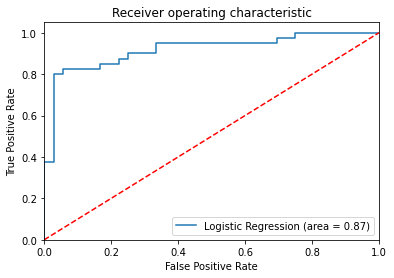
\includegraphics[width=0.5\linewidth]{LR.png}
    \caption{ROC Curve for LR}
    \label{LR}
\end{figure}

\subsection{RF Results:}
A Random Forest model was also employed for heart disease prediction. The Random Forest model achieved an accuracy of 84\%, precision of 85\% for positive cases, recall of 84\% for positive cases, and F1-score of 84\%.


\begin{table}[h!]
    \centering
    \caption{RF Performance}
    \label{tab:_ex_tab}
    \begin{tabular}{cccc}     
        \toprule
             Metric  & Value\\
        \midrule
            Accuracy  & 84\% \\
           Precision & 85\% \\
           Recall  & 84\% \\
           F1-Score & 84\% \\ 
        \bottomrule
    \end{tabular}
\end{table}

\subsection{ROC Curve for RF}

\begin{figure}[H]
    \centering
    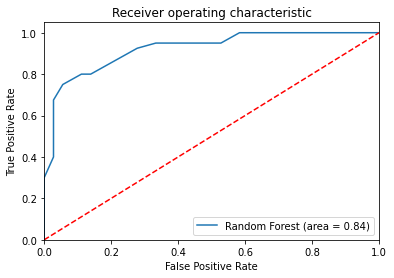
\includegraphics[width=0.5\linewidth]{RF.png}
    \caption{ROC Curve for RF}
    \label{RF}
\end{figure}

\subsection{NB Results:}
The Naive Bayes model was implemented as another approach for heart disease prediction. The Naive Bayes model achieved an accuracy of 83\%, precision of 83\% for positive cases, recall of 83\% for positive cases, and F1-score of 83\%.


\begin{table}[h!]
    \centering
    \caption{NB Performance}
    \label{tab:_ex_tab}
    \begin{tabular}{cccc}     
        \toprule
             Metric  & Value\\
        \midrule
            Accuracy  & 83\% \\
           Precision & 83\% \\
           Recall  & 83\% \\
           F1-Score & 83\% \\ 
        \bottomrule
    \end{tabular}
\end{table}

\subsection{ROC Curve for NB}

\begin{figure}[H]
    \centering
    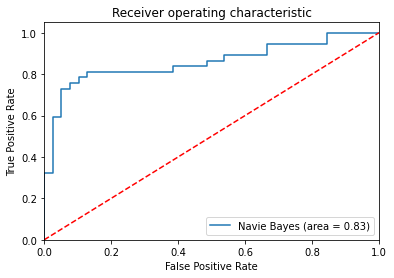
\includegraphics[width=0.5\linewidth]{NB.png}
    \caption{ROC Curve for NB}
    \label{NB}
\end{figure}

\section{Comparison of Algorithms}
Based  on the evaluation metrics, the LR model achieved the best performance in predicting heart disease. It obtained an accuracy of 87\%, indicating a high degree of correctness in its predictions. Additionally, the LR model demonstrated a good balance between precision (88\%) and recall (87\%) as reflected by the F1-score of 87\%.

While RF and NB achieved reasonable performance (around 83-84\% accuracy), LR outperformed them in terms of all chosen metrics. This could be due to the specific characteristics of the dataset or the inherent strengths of LR in handling linear relationships between features.


\section{Why Did Logistic Regression Perform Well?}
Logistic Regression demonstrated superior performance compared to Random Forest and Naive Bayes in predicting heart disease. Several factors contributed to its success:

\begin{itemize}
    \item Linear Relationship Handling: Logistic Regression is particularly effective when the relationship between features and the target variable is linear. In our dataset, features might have linear relationships with the likelihood of heart disease, which Logistic Regression can exploit effectively.
    
    \item Interpretability Logistic Regression provides interpretable results, allowing us to understand the impact of each feature on the prediction. This transparency is essential in a medical context, where understanding the factors contributing to a prediction is crucial.
    
    \item Efficient with High-Dimensional Data Logistic Regression is efficient when dealing with high-dimensional data, making it suitable for datasets with a large number of features.
\end{itemize}

\section{Interpretation of Results}

By achieving an accuracy of 87\%, Logistic Regression has demonstrated its potential as a valuable tool for early detection and risk assessment of heart disease. The balance between precision, recall, and accuracy indicates the model's effectiveness in correctly identifying patients with heart disease while minimizing false positives and false negatives.

\section{Summary}
This project explored the application of machine learning algorithms for heart disease prediction. The results demonstrate that the LR model achieved promising performance in predicting heart disease based on patient data. This approach has the potential to be a valuable tool for early detection and risk assessment of heart disease, ultimately contributing to improved patient outcomes.